\section{Exploratory Data Analysis}
\label{sec:eda}

Before building any model we looked at the data to check that it behaves the way physics says it should, and to find which inputs matter. All charts are produced by \texttt{data\_scripts/eda.py} from the merged weather table (43{,}920 hourly rows, five cities, 2024) and from the cleaned Kaggle plant data.

\subsection{Sunlight by month and city}
Figure~\ref{fig:month} shows the average daily sunlight energy for each month. All five cities follow the same shape: sunlight rises from winter to a peak in May or June, then falls again. The peak is between 7.2 and 7.5~kWh/m$^2$/day for every city (May for Islamabad, Karachi, Lahore and Multan, June for Peshawar).

The cities differ most in winter and during the monsoon. Lahore and Multan fall to about 1.7 and 1.9~kWh/m$^2$/day in January, roughly a quarter of their May values. This is consistent with winter fog and smog in the Punjab, although this chart alone does not prove the cause. Karachi stays much more even through the year; its lowest month is August (4.1~kWh/m$^2$/day), which fits the cloudy monsoon season. Over the full year, Karachi receives the most sunlight (5.31~kWh/m$^2$/day), followed by Peshawar (5.06), Islamabad (4.80), Multan (4.77) and Lahore (4.72). Two points matter for the product: location and season change the expected output a lot, so a single fixed average cannot be right for every user, and the winter dip in Lahore and Multan is exactly the kind of effect a data-driven model should capture.

\begin{figure}[H]
\centering
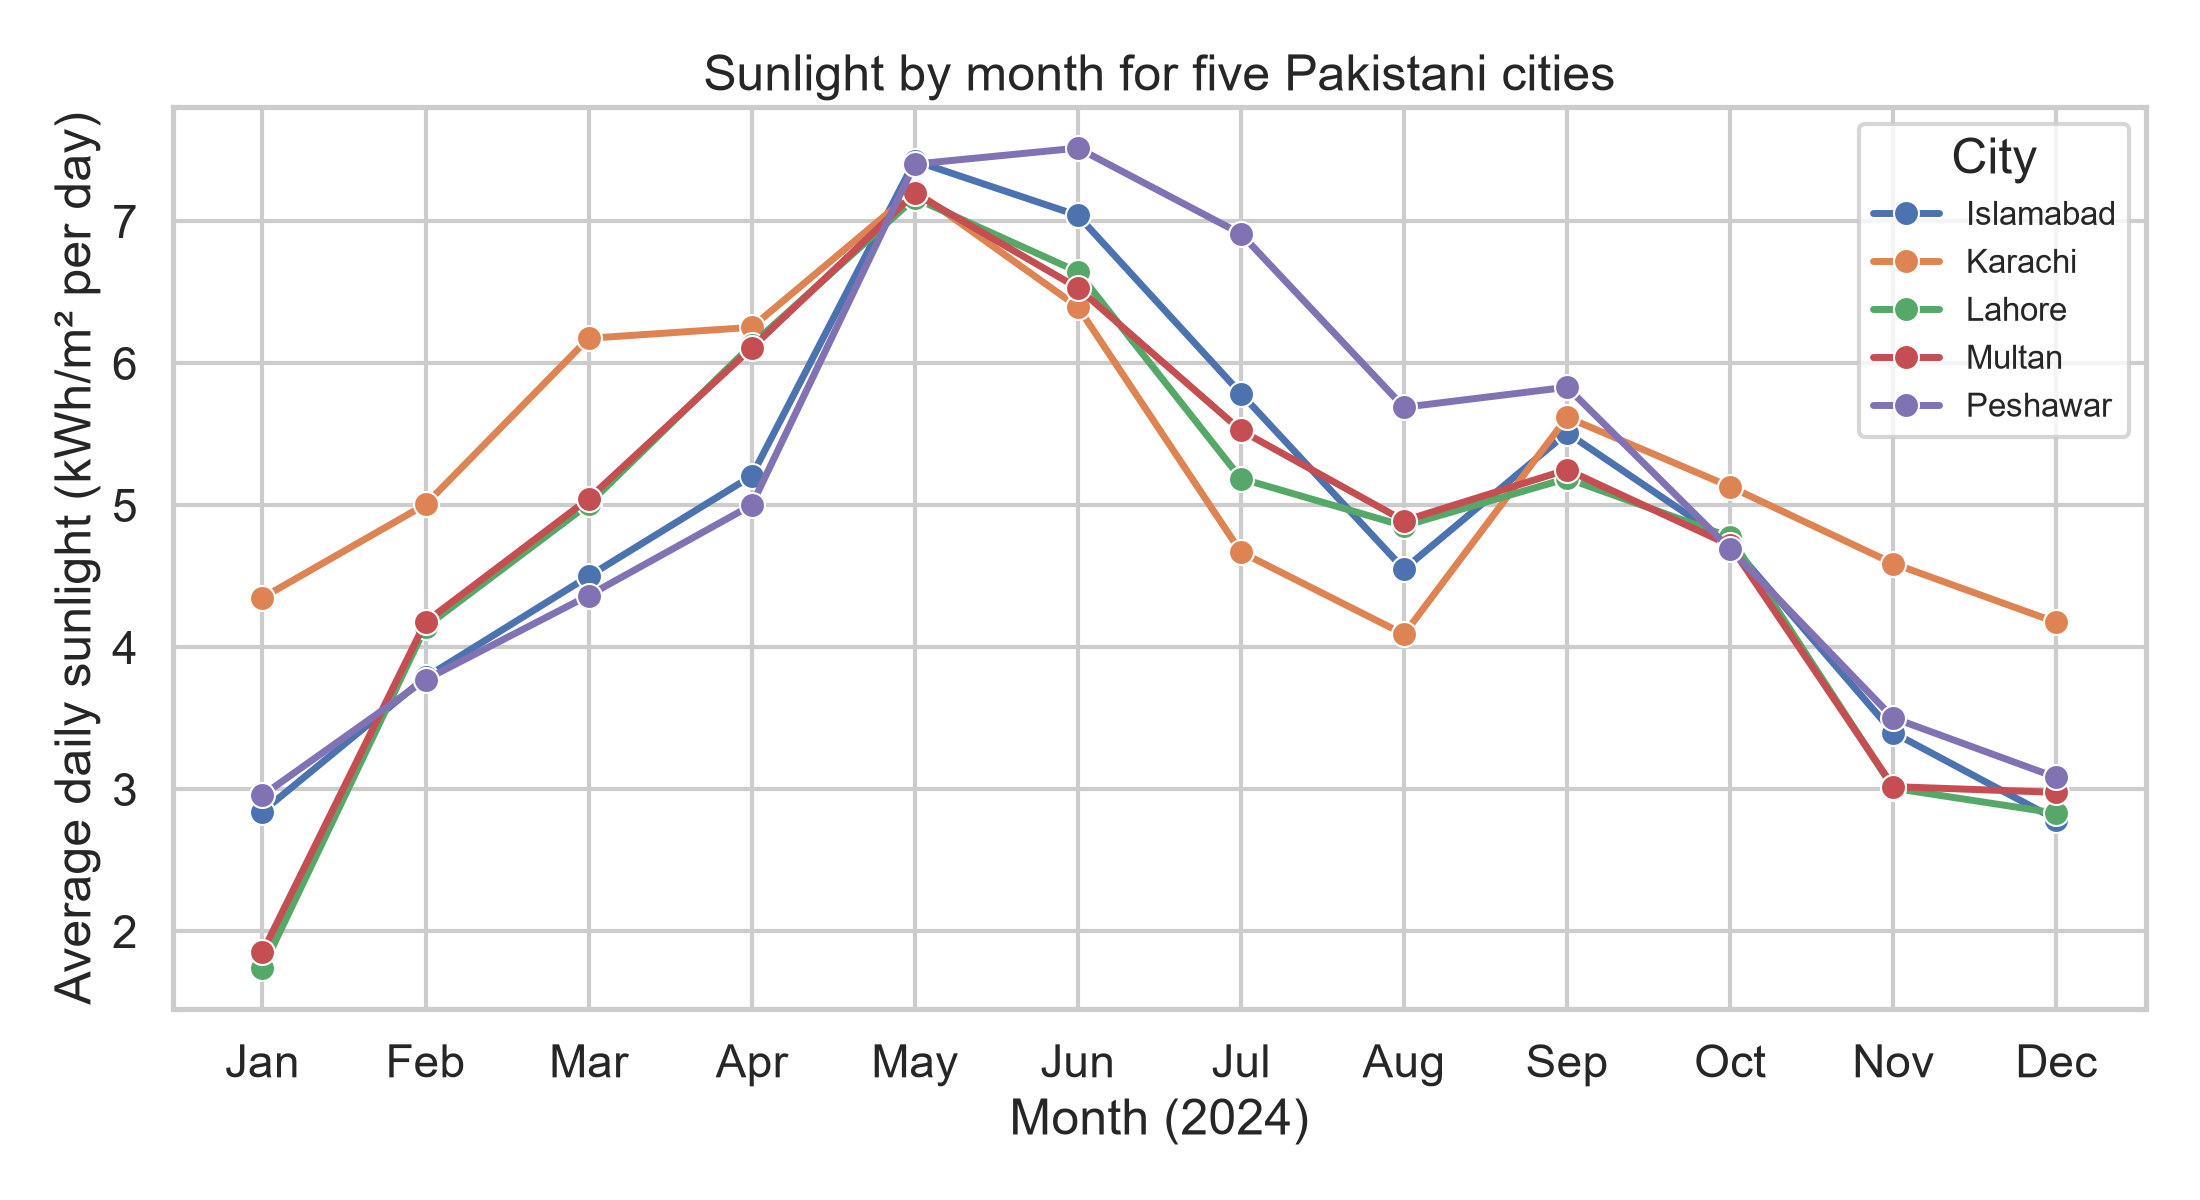
\includegraphics[width=0.88\textwidth]{01_sunlight_by_month.png}
\caption{Average daily sunlight energy by month for the five cities (2024, NASA POWER).}
\label{fig:month}
\end{figure}

\subsection{Correlation between weather features}
Figure~\ref{fig:corr} shows how the weather variables relate to each other during daytime hours (night hours are excluded, because sunlight is always zero then and would distort the picture). Sunlight is positively related to temperature ($r = 0.45$) and negatively related to humidity ($r = -0.42$): sunny hours are warmer and drier. Cloud cover and PM2.5 both reduce sunlight, but only mildly in this hour-by-hour view ($r = -0.20$ and $r = -0.18$). These links look weak because each hourly value also depends on the time of day and the height of the sun, which the correlation does not remove. They are also not strong enough to say that cloud cover or smog can be ignored; Figure~\ref{fig:cloud} isolates their effect. No pair of input variables is so strongly correlated that it would make a model unstable (the largest is $|r| = 0.45$).

\begin{figure}[H]
\centering
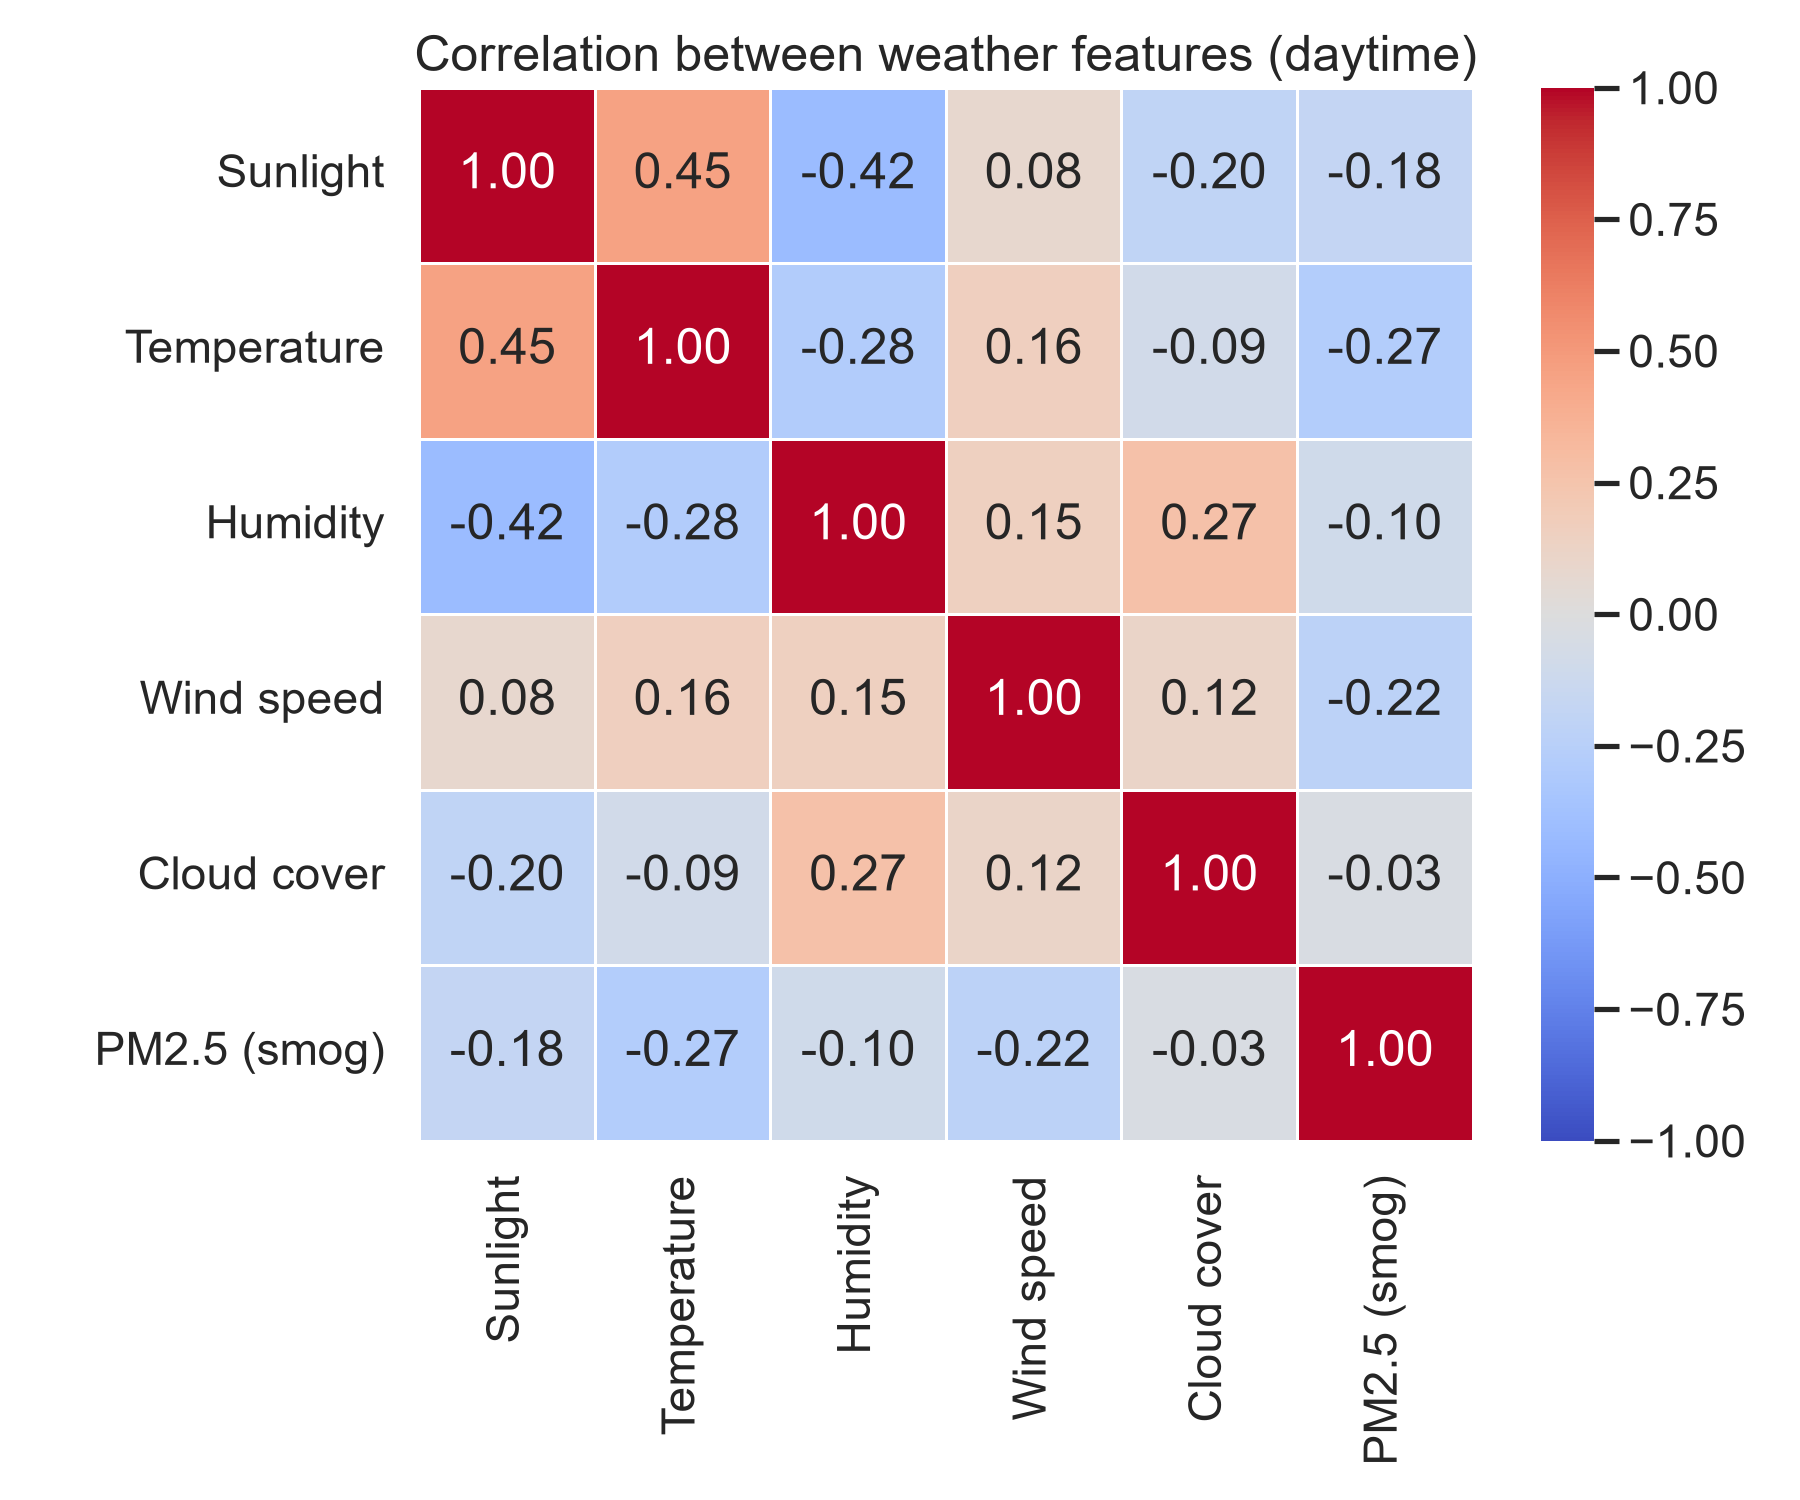
\includegraphics[width=0.72\textwidth]{02_correlation_heatmap.png}
\caption{Correlation between the weather features for daytime hours.}
\label{fig:corr}
\end{figure}

\subsection{Sunlight and panel output}
Figure~\ref{fig:output} compares sunlight with the DC power produced by the inverters in the Kaggle plant data. The two are almost perfectly linked, with a correlation of r = 0.993 across 68,711 cleaned readings. This confirms that sunlight is the main driver of solar output, so accurate sunlight forecasts will translate directly into accurate generation forecasts.

\begin{figure}[H]
\centering
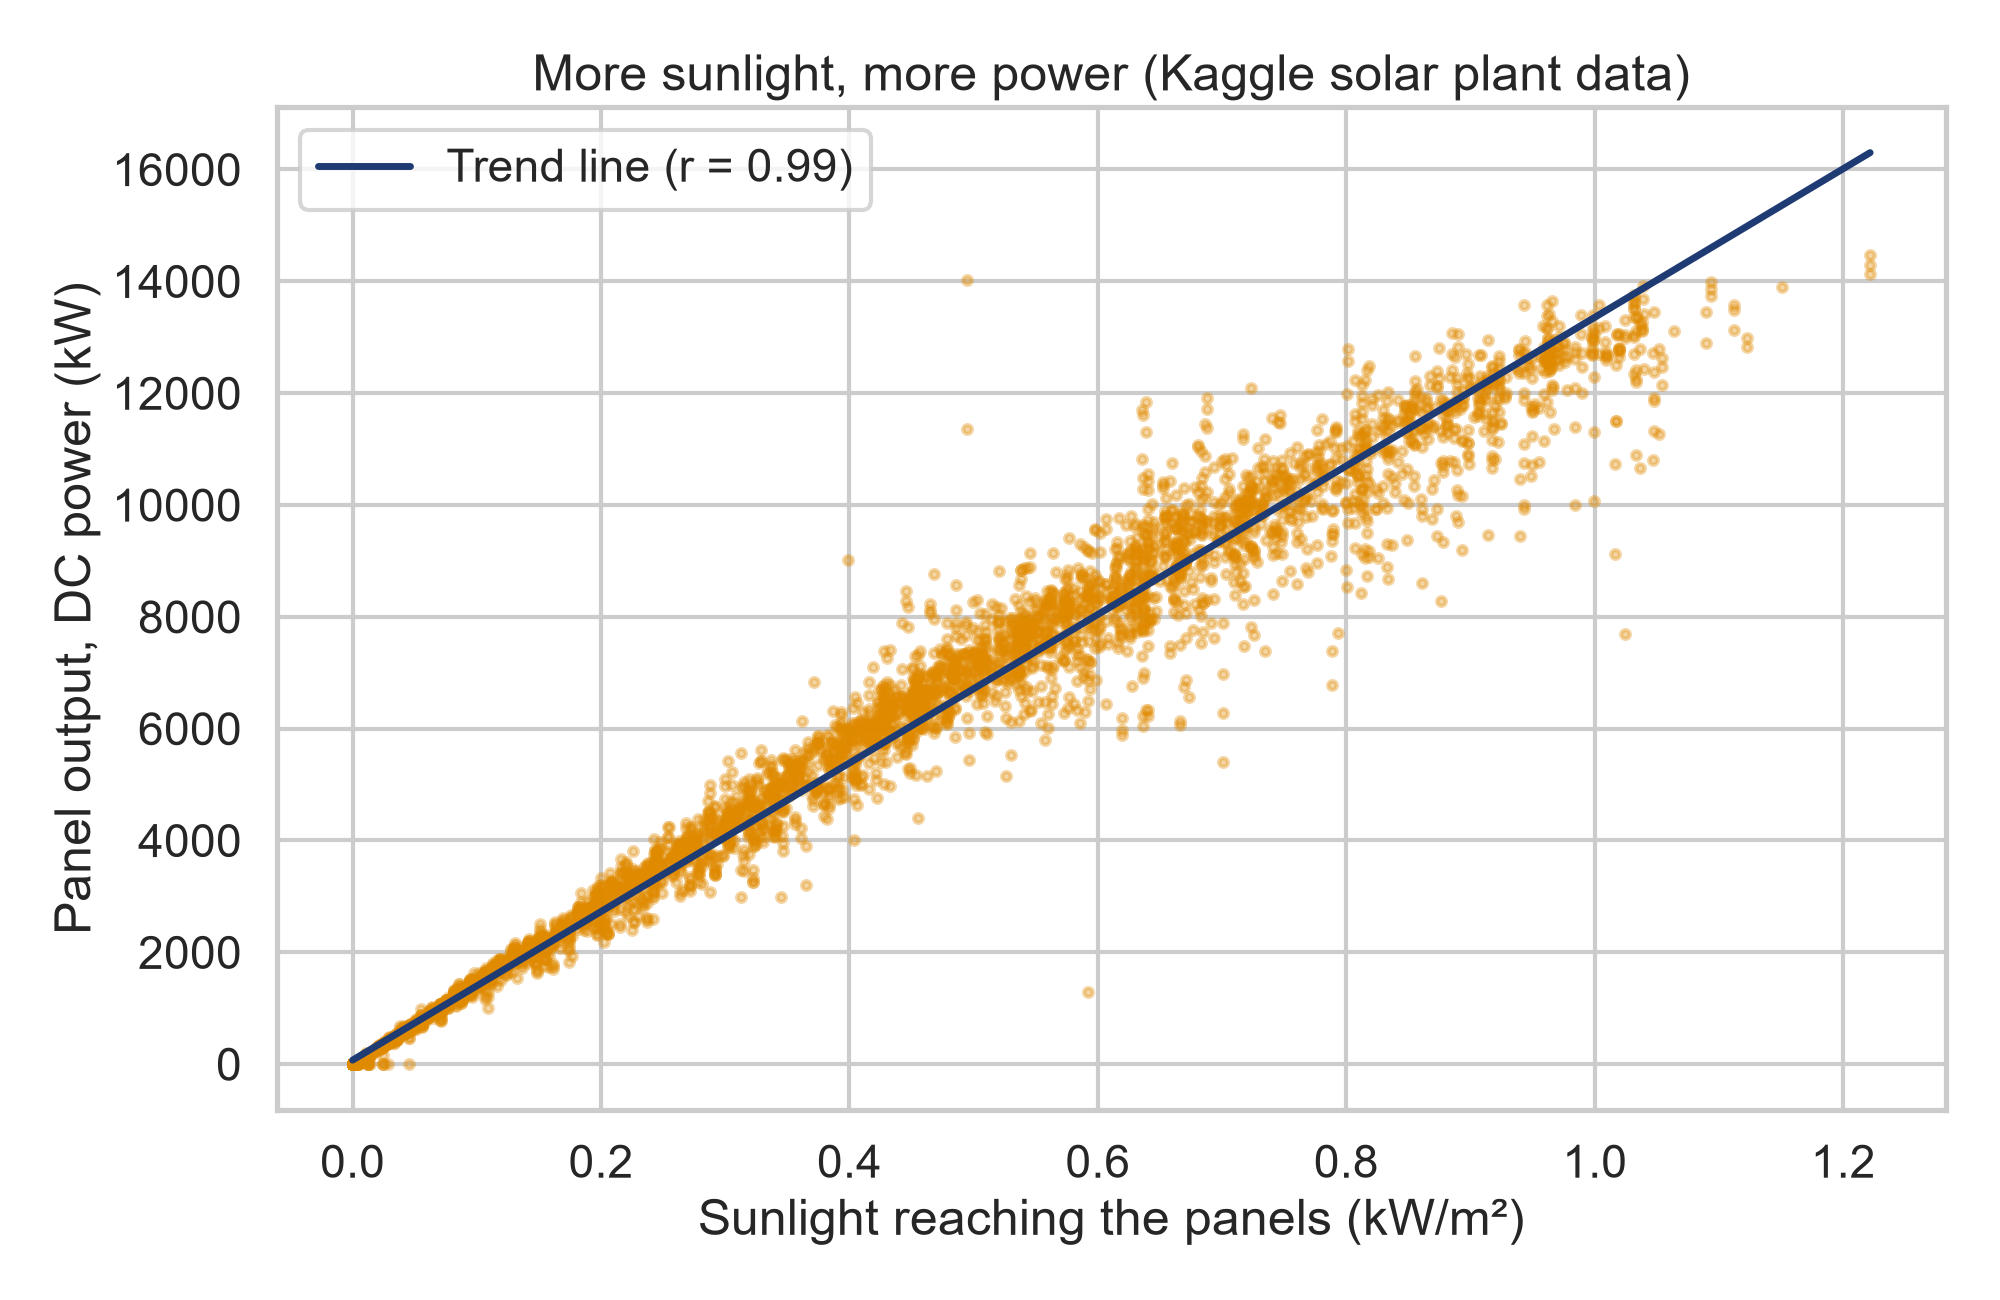
\includegraphics[width=0.8\textwidth]{03_sunlight_vs_output.png}
\caption{Sunlight against panel output (DC power) in the Kaggle solar plant data.}
\label{fig:output}
\end{figure}

\subsection{Cloud cover and sunlight}
The Kaggle plant data does not record cloud cover and comes from a different place and year, so we cannot plot cloud cover against panel output directly. Instead we show the effect in two steps: Figure~\ref{fig:cloud} shows how cloud cover changes sunlight, and Figure~\ref{fig:output} shows how sunlight changes output. For Figure~\ref{fig:cloud} we only use the hours from 11:00 to 13:00, when the sun is highest, so that the effect of the time of day is mostly removed.

Midday sunlight stays fairly steady while cloud cover rises up to about 80\%, and drops clearly under heavy overcast. At 90 to 100\% cloud cover the average is about 490~W/m$^2$, against about 730~W/m$^2$ under clear skies (below 10\% cloud), a fall of 32\%. The correlation between cloud cover and midday sunlight is moderate ($r = -0.41$). The wide spread inside each band has two main causes: the sun sits lower in winter than in summer even at midday, and cloud cover and sunlight come from two different models (Open-Meteo and NASA), which do not always agree. For the project this means cloud cover is a useful but imperfect input, and it supports using several weather inputs together instead of a single formula.

\begin{figure}[H]
\centering
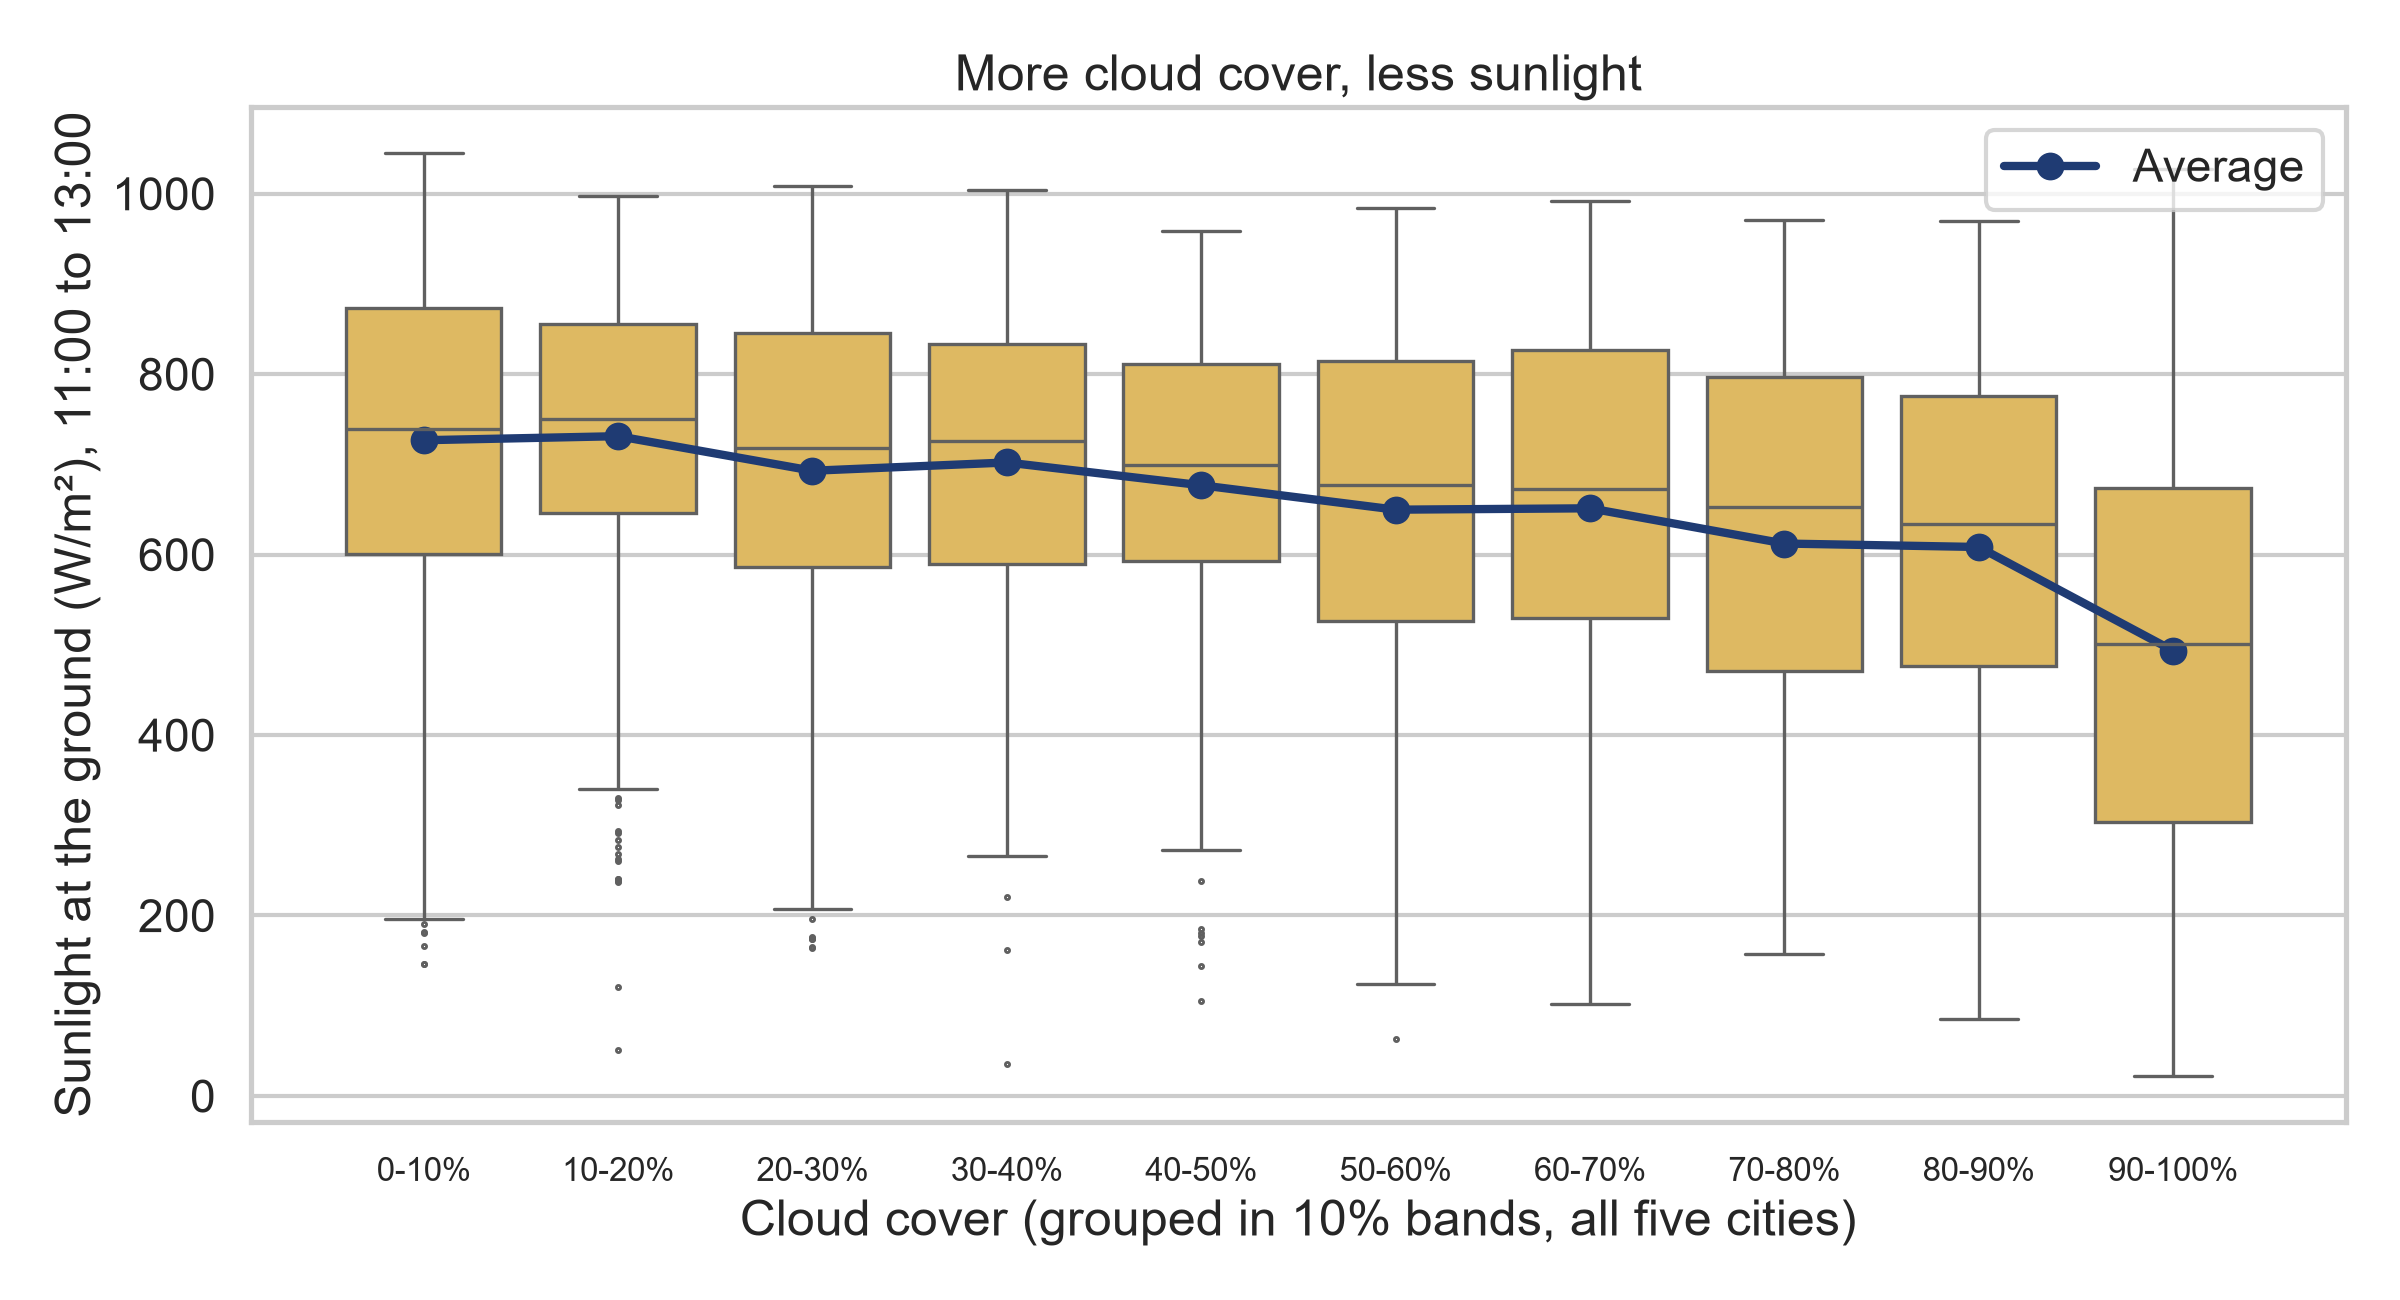
\includegraphics[width=0.88\textwidth]{04_cloud_cover_vs_sunlight.png}
\caption{Midday sunlight (11:00 to 13:00) for each 10\% band of cloud cover, all five cities. The line connects the band averages.}
\label{fig:cloud}
\end{figure}

\subsection{Missing values}
Figure~\ref{fig:missing} shows the share of missing values in each raw weather column before cleaning. We found none in the NASA POWER columns (after treating the $-999$ code as missing) or in the Open-Meteo columns, so none of these values had to be filled in. The cleaning of the Kaggle plant data (faulty inverters and invalid night readings) is described in the Data Cleaning section.

\begin{figure}[H]
\centering
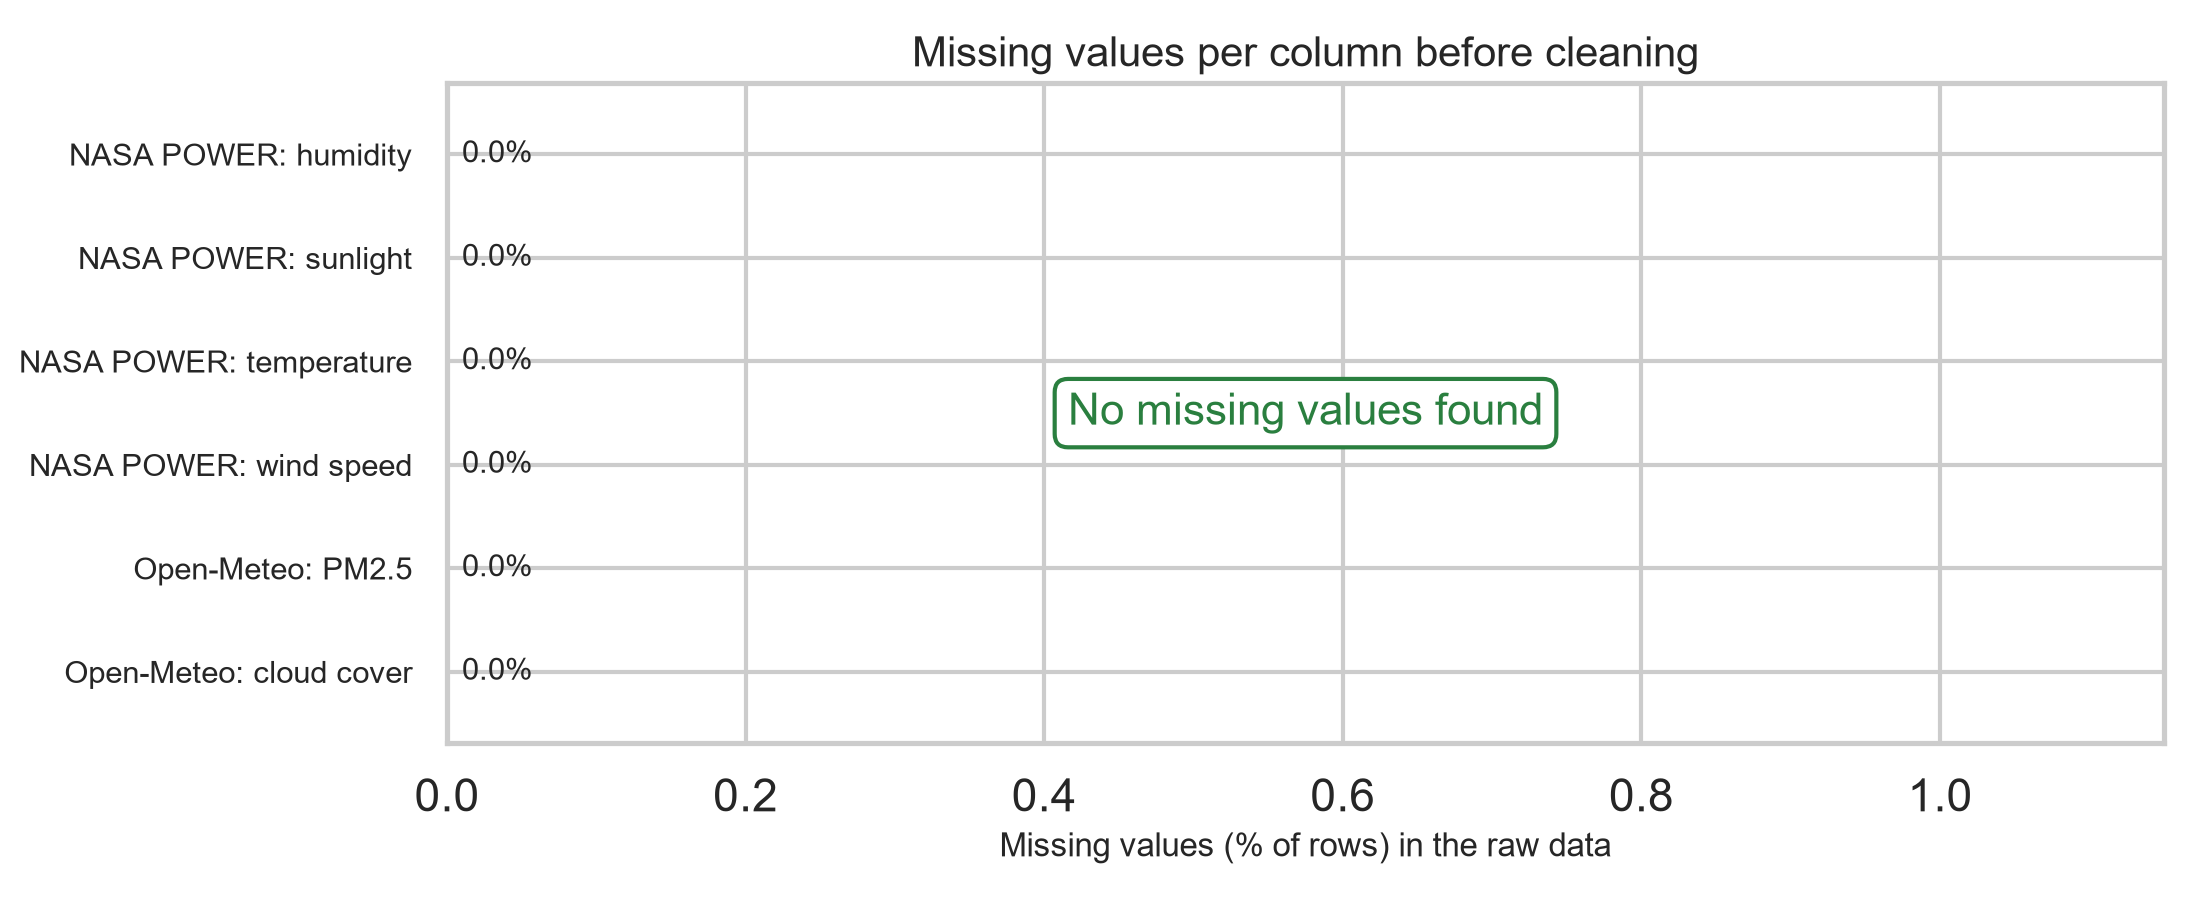
\includegraphics[width=0.85\textwidth]{05_missing_values.png}
\caption{Missing values per column in the raw data.}
\label{fig:missing}
\end{figure}

\subsection{What the analysis tells us}
Sunlight is the main driver of output and varies strongly by month and city. Temperature, humidity, cloud cover and smog each have a smaller effect, and they act together, which supports using a machine learning model with all of them as inputs. The city must also be an input, and this is why we one hot encode it.